\title{Chum Populations}

\documentclass[12pt,  one column]{article}
\usepackage{graphicx}
\usepackage{float}

\begin{document}

Does this turn into two papers?

 - linkage map and individual-based analyses - including duplicated loci

 - inference of adaptation - life history variation  - Fst across the genome.  
 

\section*{Abstract}
To do

\section*{Introduction}
To do

Expected population structure

ESA listing - summer chum ESU

Salmonid WGD

\section*{Methods}

\subsection*{Linkage map}

Sequence analysis and genotyping

Identification of paralogs follows Waples (2015)

Map construction follows Waples (2015)

Synteny - relation to genetic resources
\begin{itemize}
	\item Chinook salmon
    \item Atlantic salmon
\end{itemize}

\subsection*{Population Genetics}
Sequence analysis and genotyping

Genotyping duplicate loci using the dominance coding suggested by Patterson (2006). 
Individual-based analyses
\begin{itemize}
	\item PCAs - How do compare? - maybe measure info loss?
    \item Heterozygosity
	\item Fst across the genome
\end{itemize}

Population-based analyses
\begin{itemize}
	\item MAF, Heterozygosity
	\item Fst across the genome
    \item Effective population size - Waples and Do
    \item Bayescan outlier tests
\end{itemize}

\section*{Results}

\subsection*{Linkage map}
Identification of paralogs

congruence of paralog across families (supplemental table)

Consensus linkage map

Table (Figure?)
placement of centromeres

table (supplemental)
paralogs
note the distribution of paralogs matches the  pattern found in other salmonids
syntenic relationships - per LG
Table (supplemental?)


\subsection*{Population Genetics}

Summarize population relationships
Figure of individual-based 4 PCAs

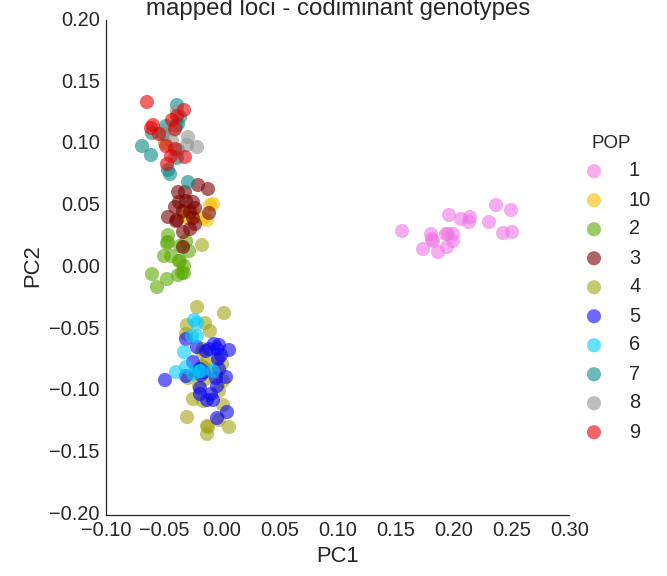
\includegraphics[scale=.3]{figures/PCA_codom.png}
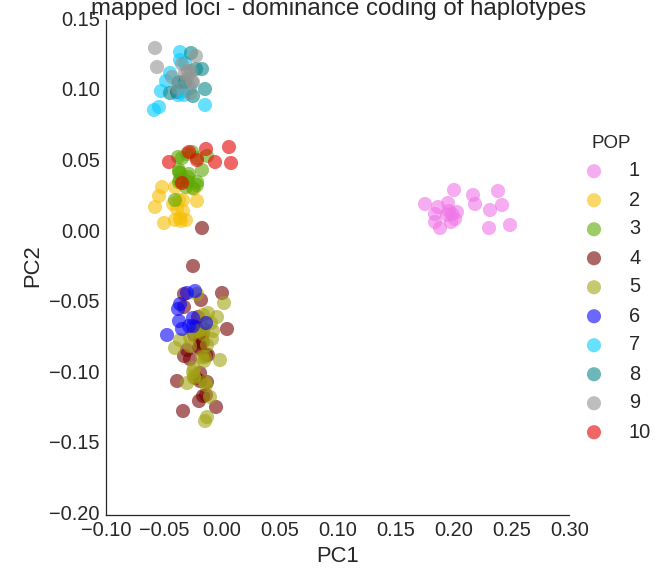
\includegraphics[scale=.3]{figures/PCA_dom.png}

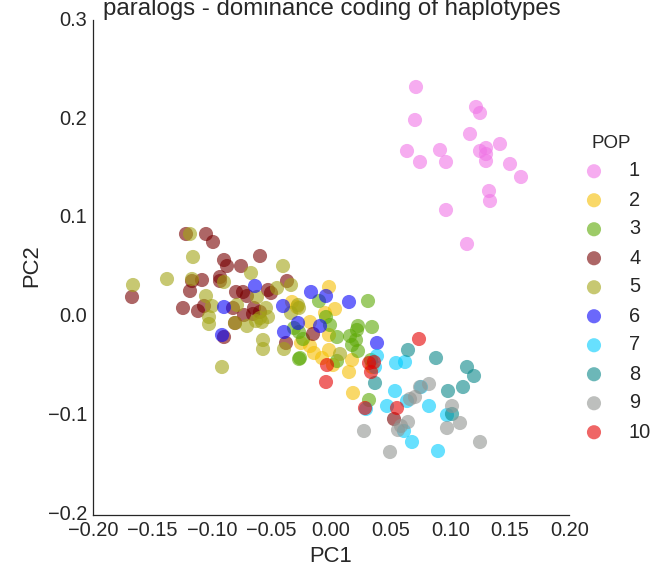
\includegraphics[scale=.3]{figures/PCA_dom_paralogs.png}
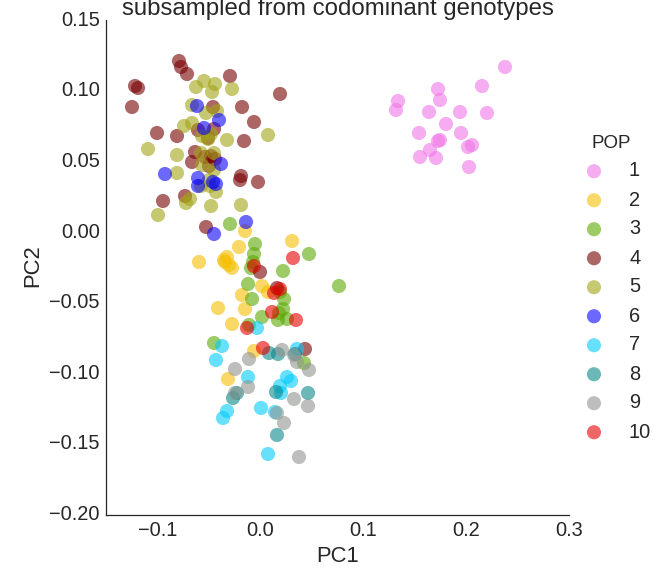
\includegraphics[scale=.3]{figures/PCA_codom_subsample.png}
\subsection*{Population Genetics}



measure information loss from dominance coding
discuss population vs individual based results
paralogs have similar neutral patterns of population structure.
can we demonstrate contained within paralogs by bootstrapping 
Genome scans (Outliers) - LG regions highlighted.

\subsection*{Effective population size}

\subsection*{Ascertainment Bias}
Demonstrate ascertainment effect when using only loci on linkage map - effect on allele frequencies.


\section*{Discussion}
To do

\section*{Supplemental}

\begin{figure}[H]
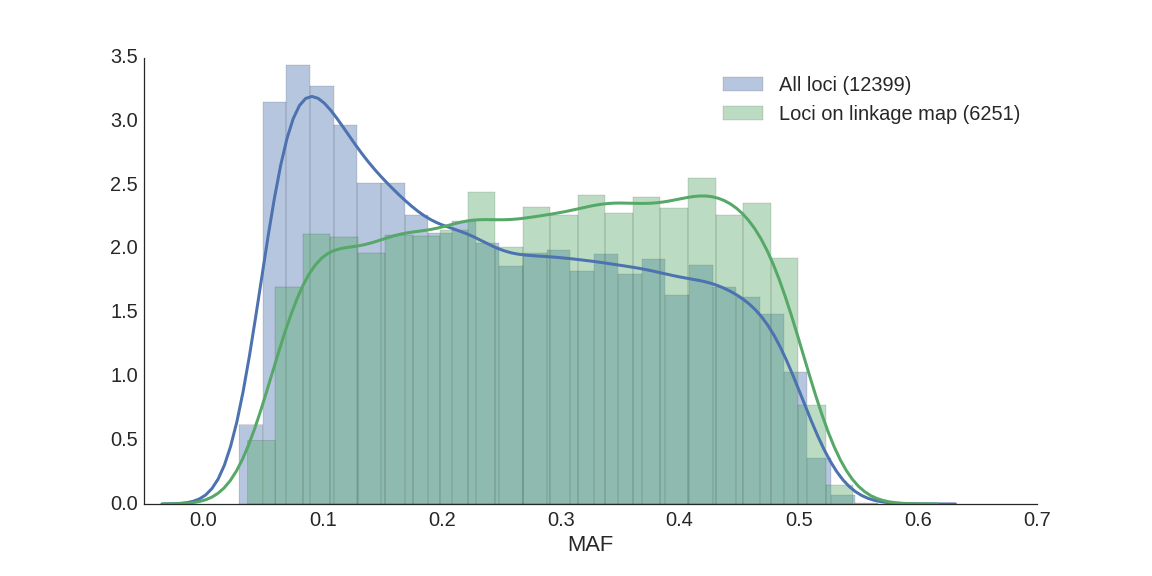
\includegraphics[scale=.3]{figures/supplemental/ascertainment.png}
\caption{Minor allele frequency distribution for all genotyped loci (blue) and just the loci placed on the linkage map (green). The increase in MAF shows the effect of ascertainment bias.}
\end{figure}

\begin{figure}[H]
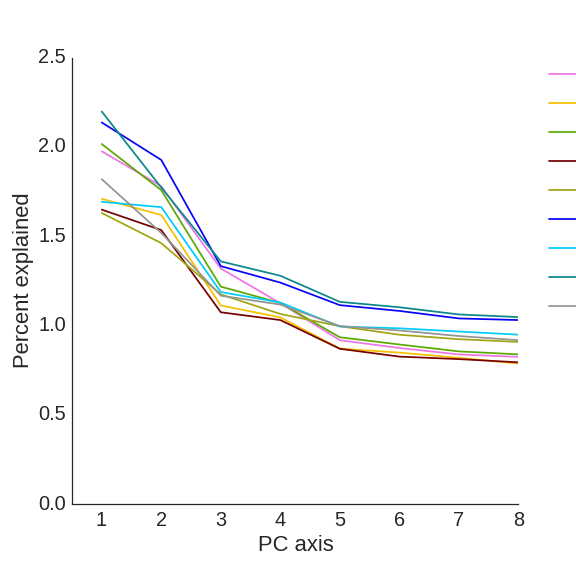
\includegraphics[scale=.4]{figures/supplemental/PCA_eigenvalues.png}
\caption{Percent variance explained (eigenvalue) for the first eight PC axes of each locus set.  Notice the similarity between the two bi-allelic sets and the two haplotypic sets.}
\end{figure}

\begin{figure}[H]
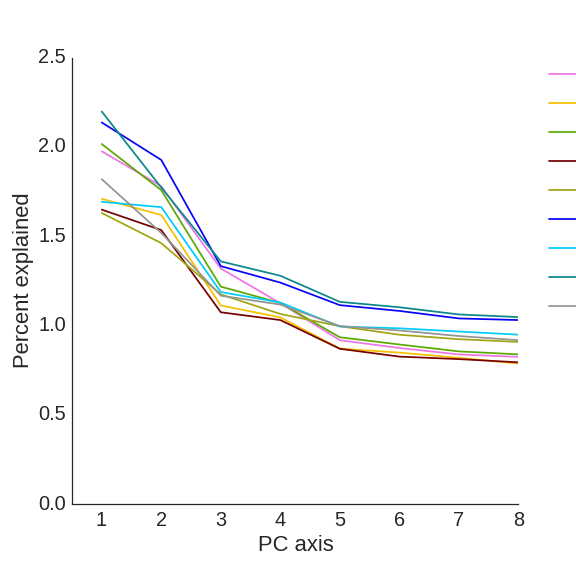
\includegraphics[scale=.4]{figures/supplemental/PCA_eigenvalues.png}
\caption{Percent variance explained (eigenvalue) for the first eight PC axes of each locus set.  Notice the similarity between the two bi-allelic sets and the two haplotypic sets.}
\end{figure}

\begin{figure}[H]
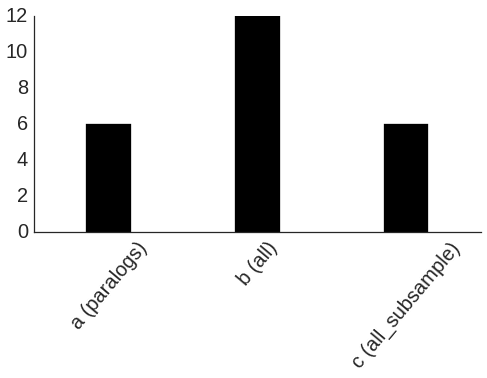
\includegraphics[scale=.4]{figures/supplemental/TW_stats.png}
\caption{Number of significant PC axes as determined by the Tracey-Widom test.}
\end{figure}

\begin{figure}[H]
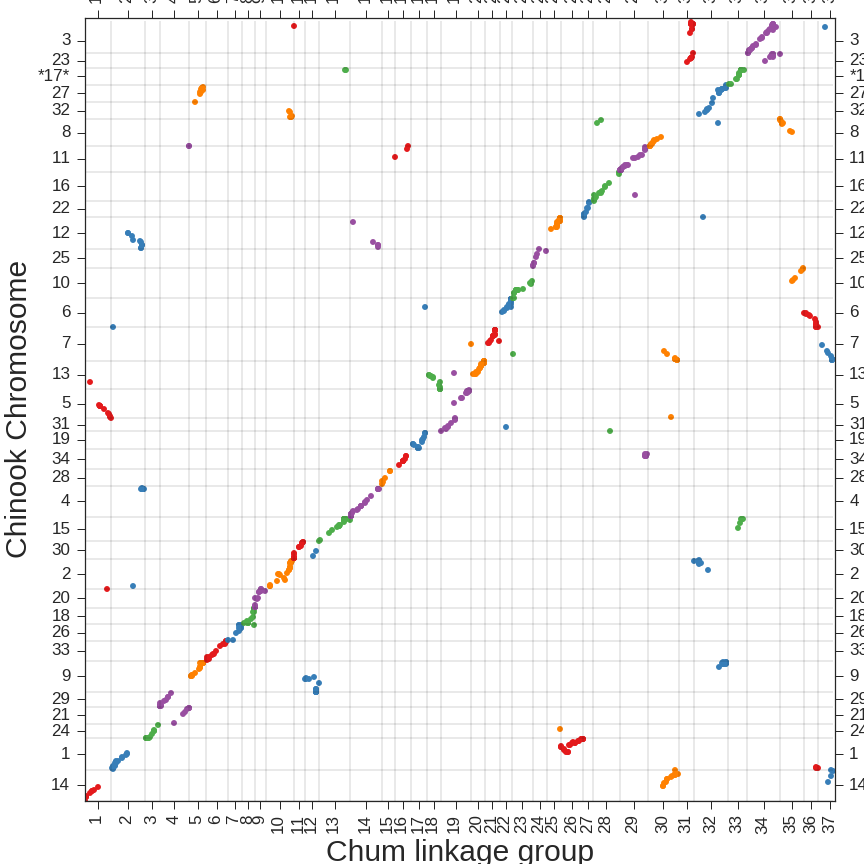
\includegraphics[scale=.4]{figures/supplemental/synteny_chinook.png}
\caption{Oxford grid - Chum and Chinook linkag groups.}
\end{figure}

%\begin{figure}
%\begin{center}
%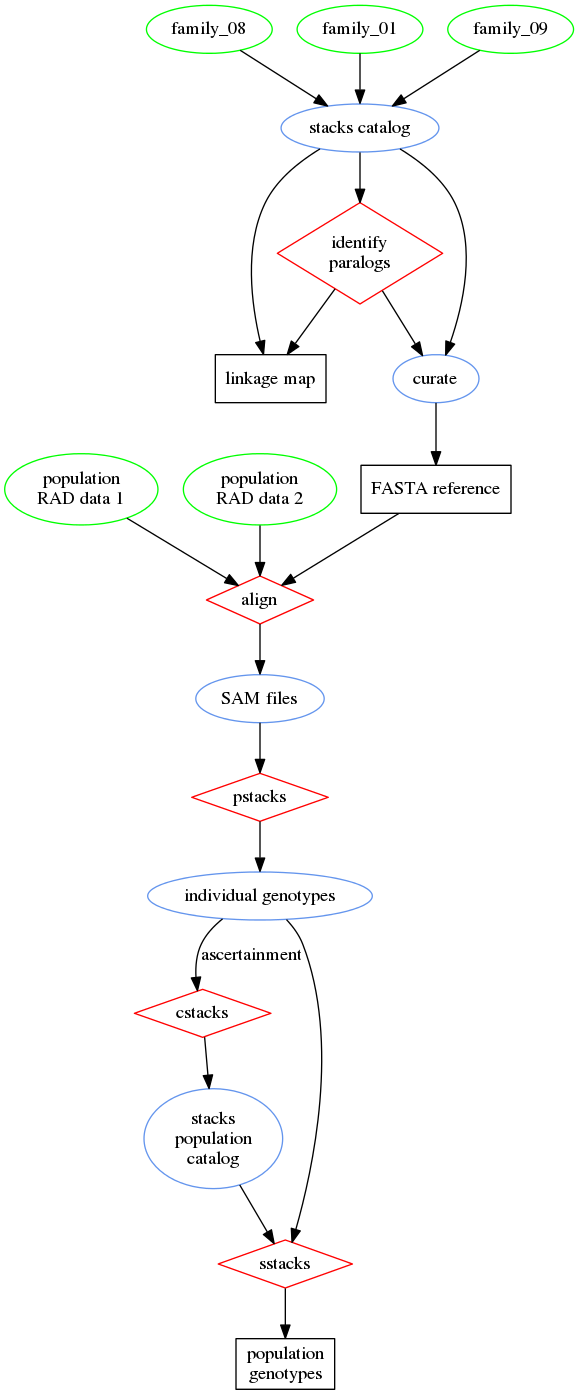
\includegraphics[scale=.3]{figures/supplemental/analysis_flowchart.png}
%\end{center}
%\end{figure}


\end{document}